\documentclass[twoside,11pt,fleqn,noabs]{starlink}

% ? Specify used packages
% ? End of specify used packages

% -----------------------------------------------------------------------------
% ? Document identification
% Fixed part
\stardoccategory    {Starlink Cookbook}
\stardocinitials    {SC}
\stardocsource      {sc\stardocnumber}
\stardoccopyright
{Copyright \copyright\ 1997 Science and Technology Facilities Council}

% Variable part - replace [xxx] as appropriate.
\stardocnumber      {10.1}
\stardocauthors   {J.~A. Stevens, R.~J. Ivison, T. Jenness\\
                                Joint Astronomy Centre, Hilo, Hawaii}
\stardocdate        {1 August 1997}
\startitlepic{
\includegraphics[width=2.0in]{sc10_logo}}
\stardoctitle       {The SCUBA photometry cookbook}
% ? End of document identification
% -----------------------------------------------------------------------------

% ? Document specific \providecommand or \newenvironment commands.

% A new environment for quoting verbatim
% Environment for indenting and using a small font.
\newenvironment{myquote}{\begin{quote}\begin{small}}{\end{small}\end{quote}}

\providecommand{\text}[1]{{\small \tt #1}}

% Starlink Package names
\providecommand{\starlink}{\htmladdnormallink{Starlink}{http://www.starlink.ac.uk/}}

% set up some common package names
\providecommand{\Kappa}{\xref{\textsc{Kappa}}{sun95}{}}
\providecommand{\Figaro}{\xref{\textsc{Figaro}}{sun86}{}}
\providecommand{\gaia}{\xref{\textsc{Gaia}}{sun214}{}}
\providecommand{\convert}{\xref{\textsc{Convert}}{sun55}{}}
\providecommand{\fluxes}{\xref{\textsc{Fluxes}}{sun213}{}}
\providecommand{\Iras}{\xref{\textsc{Iras90}}{sun163}{}}
\providecommand{\ndf}{\xref{NDF}{sun33}{}}
\providecommand{\agi}{\xref{AGI}{sun48}{}}
\providecommand{\surf}{\xref{\textsc{Surf}}{sun216}{}}

% Application tasks
\providecommand{\task}[1]{\textsf{#1}}

% ADAM parameters
\providecommand{\param}[1]{\texttt{#1}}

% SURF tasks
\providecommand{\rebin}{\xref{\task{rebin}}{sun216}{REBIN}}
\providecommand{\bolrebin}{\xref{\task{bolrebin}}{sun216}{BOLREBIN}}
\providecommand{\intrebin}{\xref{\task{intrebin}}{sun216}{INTREBIN}}
\providecommand{\chgqual}{\xref{\task{change\_quality}}{sun216}{CHANGE_QUALITY}}
\providecommand{\chgflat}{\xref{\task{change\_flat}}{sun216}{CHANGE_FLAT}}
\providecommand{\chgpnt}{\xref{\task{change\_pointing}}{sun216}{CHANGE_POINTING}}
\providecommand{\chgdata}{\xref{\task{change\_data}}{sun216}{CHANGE_DATA}}
\providecommand{\resw}{\xref{\task{reduce\_switch}}{sun216}{REDUCE_SWITCH}}
\providecommand{\flatf}{\xref{\task{flatfield}}{sun216}{FLATFIELD}}
\providecommand{\skydip}{\xref{\task{skydip}}{sun216}{SKYDIP}}
\providecommand{\scuphot}{\xref{\task{scuphot}}{sun216}{SCUPHOT}}
\providecommand{\ext}{\xref{\task{extinction}}{sun216}{EXTINCTION}}
\providecommand{\scuquick}{\xref{\task{scuquick}}{sun216}{SCUQUICK}}
\providecommand{\scuhelp}{\xref{\task{scuhelp}}{sun216}{SCUHELP}}
\providecommand{\remsky}{\xref{\task{remsky}}{sun216}{REMSKY}}
\providecommand{\scuover}{\xref{\task{scuover}}{sun216}{SCUOVER}}
\providecommand{\extdata}{\xref{\task{extract\_data}}{sun216}{EXTRACT_DATA}}
\providecommand{\sculog}{\xref{\task{sculog}}{sun216}{SCULOG}}
\providecommand{\scucat}{\xref{\task{scucat}}{sun216}{SCUCAT}}
\providecommand{\photsum}{\xref{\task{photsum}}{sun216}{PHOTSUM}}
\providecommand{\mapsum}{\xref{\task{mapsum}}{sun216}{MAPSUM}}
\providecommand{\pointsum}{\xref{\task{pointsum}}{sun216}{POINTSUM}}
\providecommand{\qdraw}{\xref{\task{qdraw}}{sun216}{QDRAW}}
\providecommand{\sigclip}{\xref{\task{sigclip}}{sun216}{SIGCLIP}}
\providecommand{\restore}{\xref{\task{restore}}{sun216}{RESTORE}}
\providecommand{\sdip}{\xref{\task{sdip}}{sun216}{SDIP}}
\providecommand{\scupa}{\xref{\task{scupa}}{sun216}{SCUPA}}
\providecommand{\obssum}{\xref{\task{obssum}}{sun216}{OBSSUM}}

% Non surf tasks

\providecommand{\display}{\xref{\task{display}}{sun95}{DISPLAY}}
\providecommand{\linplot}{\xref{\task{linplot}}{sun95}{LINPLOT}}
\providecommand{\drawsig}{\xref{\task{drawsig}}{sun95}{DRAWSIG}}
\providecommand{\centroid}{\xref{\task{centroid}}{sun95}{CENTROID}}
\providecommand{\setaxis}{\xref{\task{setaxis}}{sun95}{SETAXIS}}
\providecommand{\kstest}{\xref{\task{kstest}}{sun95}{KSTEST}}
\providecommand{\stats}{\xref{\task{stats}}{sun95}{STATS}}
\providecommand{\thresh}{\xref{\task{thresh}}{sun95}{THRESH}}
\providecommand{\setbb}{\xref{\task{setbb}}{sun95}{SETBB}}
\providecommand{\fitslist}{\xref{\task{fitslist}}{sun95}{FITSLIST}}
\providecommand{\ndffits}{\xref{\task{ndf2fits}}{sun55}{NDF2FITS}}
\providecommand{\ndfascii}{\xref{\task{ndf2ascii}}{sun55}{NDF2ASCII}}
\providecommand{\cadd}{\xref{\task{cadd}}{sun95}{CADD}}
\providecommand{\cdiv}{\xref{\task{cdiv}}{sun95}{CDIV}}
\providecommand{\add}{\xref{\task{add}}{sun95}{ADD}}
\providecommand{\hdstrace}{\xref{\task{hdstrace}}{sun102}{}}
\providecommand{\psmerge}{\xref{\task{psmerge}}{sun164}{}}
\providecommand{\wdfits}{\xref{\task{wdfits}}{sun86}{WDFITS}}
\providecommand{\delobj}{\xref{\task{delobj}}{sun86}{DELOBJ}}
\providecommand{\setvar}{\xref{\task{setvar}}{sun95}{SETVAR}}
\providecommand{\ndfcopy}{\xref{\task{ndfcopy}}{sun95}{NDFCOPY}}
\providecommand{\gdset}{\xref{\task{gdset}}{sun95}{GDSET}}
\providecommand{\flip}{\xref{\task{flip}}{sun95}{FLIP}}
\providecommand{\image}{\xref{\task{image}}{sun86}{IMAGE}}

% ? End of document specific commands
% -----------------------------------------------------------------------------
%  Title Page.
%  ===========
\begin{document}
\scfrontmatter

\section{Introduction}

This document describes the basic reduction of photometric data taken with the
Submillimetre Common-User Bolometer Array (SCUBA) at the
\htmladdnormallink{James Clerk Maxwell
Telescope}{http://www.jach.hawaii.edu/JCMT/}. The adopted method is applicable
to the full range of SCUBA's photometric observing modes: simple `stare' type
observations such as those performed with UKT14, small jiggle maps taken with
a single pixel or either of the above but chopping between 2 or 3 bolometers
on the arrays.

At the time of writing the fully commissioned photometry mode employs
a single bolometer to make small 9-point maps centred on the
source. This scheme has been shown to give better signal-to-noise
under moderate submillimetre `seeing' conditions than the traditional
`stare' method.  However, the reduction procedure is still valid
regardless of the adopted jiggle mode, for example, if a 7-point map
or a scheme with no jiggling was used for the observation.  Although
not yet fully commissioned, it is possible to chop between two or
three bolometers on the arrays and the reduction of these data is
discussed briefly.  In the future more elaborate methods, such as two
and three position chopping, will be available and the document will
evolve accordingly.  For a more detailed discussion of photometric
observing modes with SCUBA see, for example, the
\htmladdnormallink{SCUBA Observing
Manual}{http://www.jach.hawaii.edu/jcmt_sw/scuba/}
\cite{obsguide}.

Our basic philosophy was to style the SCUBA photometry reduction
graphical interface in a manner similar to that used for UKT14 \cite{ukt14}
(i.e. \texttt{COADD}) but the observing modes and hence steps in the
reduction process are particular to SCUBA.

This cookbook requires access to the Scuba User Reduction Facility (\surf) software
\cite{surf} (for processing demodulated SCUBA data), \Kappa \cite{kappa}\footnote{This
document assumes access to at least Version 0.10 of KAPPA.} (for data display
and post-processing) and \convert\cite{convert} (for exporting data to ASCII or FITS).
\surf\ is available from the \surf\
\htmladdnormallinkfoot{homepage}{http://www.jach.hawaii.edu/jcmt\_sw/scuba/surf/}
and additionally all these packages are available from the
\htmladdnormallinkfoot{Starlink software store}{http://www.starlink.ac.uk/cgi-store/storetop}
or on the \htmladdnormallink{Starlink}{http://www.starlink.ac.uk} CD-ROM distribution.

\section{Running up the software}

The Scuba User Reduction Facility (\surf) software can be loaded
by simply typing:

\begin{small}
\begin{terminalv}
% surf

   SURF - SCUBA User Reduction Facility
     Commands are now available -- (Version 1.0-0)

     Type scuhelp for help on SURF commands.
     Type "showme sun216" to browse the hypertext documentation.
\end{terminalv}
\end{small}
\section{The \texttt{SURF} commands}

The SCUBA data reduction commands are summarized briefly in this
section. On-line help for these commands can be accessed with \scuhelp\
or by replying with ?? at any prompt.

There are six steps which need to be followed in order to produce the final
coadded, but still uncalibrated, photometric result, namely \resw, \chgflat,
\flatf, \ext, \scuphot\ and \scucat. In addition, data taken with the arrays
may be corrected for sky noise variations by subtracting off the signal from
surrounding bolometers using the \remsky\ command. -- see later in this
section for a description of these commands.

The data reduction software takes the demodulated data as input and
the format is yyyymmdd\_dem\_xxxx without the \mbox{.sdf} extension,
for example, 19970711\_dem\_0025.  Additional files called
yyyymmdd\_red\_xxxx\mbox{.sdf} are produced by the on-line data reduction
software and include preliminary signal information.

The SCUBA log command, \sculog\footnote{Use \obssum\ for one line summaries},
can be run to give a log of all the observations in a directory.
All the journal software (\sculog, \obssum, \photsum, etc.)
as well as \resw\ and \skydip\ recognise the concept of a data
directory. This means that the data (demodulated or reduced) does not need
to be present in the current directory -- the tasks will search for data in the
directory specified by the \textsc{datadir} environment variable as well as
the current directory. Using the unix C-shell this can be achieved by:
\begin{terminalv}
% setenv DATADIR /wherever/data/19970706/dem
\end{terminalv}
which would instruct \obssum, say, to search for data in directory
\texttt{/wherever/data/19970706\-/dem}.
Help on the log commands
can be accessed with the \texttt{-h} option:

\begin{small}
\begin{terminalv}
% sculog -h

Usage:
  sculog [-h] [-all]
Options:
  -h[elp]        This message
  -summary       Gives a one line summary of each file
  -all           Catalog all sdf files regardless of numeric range
  -begin nn      First scan number to be considered
  -end nn        Final scan number to be considered
  -demod         Only look at raw demodulated data files (ie _dem_)
  -reduced       Only look at files reduced on-line (ie _red_)
  -mode obs      Select observation modes

also
  --begin=nn     First scan number (note the -- prefix)
  --end=nn       Final scan number
  --mode=obs     Select observation modes

  Where nn is an integer and 'obs' is a comma delimited list of obsmodes.
  Use 'perldoc sculog' for more information.
Author:
  Tim Jenness (timj@jach.hawaii.edu)
\end{terminalv}
\end{small}

The \photsum\ command uses \sculog\ to produce a brief description
of each observation (like \texttt{usum} for UKT14). If the reduced data
files are present then this summary will include signal and
\xref{skydip}{sun216}{skydips} tau values, e.g.,
\begin{small}
\begin{terminalv}
% photsum -all -reduced
 #    HST    Source   Meas/Int  Am   Filter  SubInst Signal   S/N   Tau  Seeing
---  -----   -------  -------- ---- -------- ------- ------  -----  ---  ------
42   20:17   mars        1/5   1.09 450N:850 LONG   4.80e+00 279.5  0.052 1.376
                                             SHORT  3.10e-01 8.32
45   20:30   mars        1/5   1.07 450N:850 LONG   4.85e+00 375.7  0.044 1.376
                                             SHORT  1.69e+00 185.
46   20:33   mars        1/5   1.07 450N:850 LONG   4.86e+00 275.6  0.044 1.376
                                             SHORT  1.71e+00 116.
47   20:36   mars        1/5   1.06 350N:750 LONG   4.15e+00 518.0  0.045 1.376
                                             SHORT  5.35e-01 242.
48   20:40   mars        1/5   1.06 850S:PHO P1350  4.95e+00 458.5  0.045 0.487
49   20:43   mars        1/5   1.05 850S:PHO P2000  4.22e-01 282.9  0.045 0.487
**************
50   20:46   SKYDIP     10/20       450N:850 SHORT:  0.936          0.062 0.487
                                             LONG    0.211
--------------
**************
51   20:54   SKYDIP     10/20       350N:750 SHORT:  0.943          0.062 0.487
                                             LONG    0.411
--------------
64   22:38   B21122+390  1/20  1.08 850S:PHO P2000  2.74e-06 0.203  0.048 0.17
65   22:49   B21122+390  1/20  1.09 850S:PHO P2000  2.12e-05 1.786  0.044 0.124
66   22:59   B21122+390  1/20  1.10 850S:PHO P2000  2.50e-05 2.249  0.045 0.124
67   23:09   B21122+390  1/20  1.12 850S:PHO P2000  1.79e-05 1.829  0.047 0.124
68   23:19   B21122+390  1/20  1.13 850S:PHO P1350  1.14e-04 5.434  0.05  0.098
69   23:30   B21122+390  1/20  1.15 850S:PHO P1350  1.18e-04 5.280  0.047 0.098
72   23:47   mars        1/5   1.20 850S:PHO P2000  4.19e-01 415.3  0.046 0.096
73   23:51   mars        1/5   1.21 850S:PHO P1350  4.65e+00 720.6  0.046 0.096
74   23:55   mars        1/5   1.23 450N:850 LONG   4.93e+00 548.5  0.046 0.096
                                             SHORT  1.69e+00 187.
76   00:55   mars        1/5   1.53 350N:750 LONG   4.01e+00 633.3  0.051 0.144
                                             SHORT  4.51e-01 514.
78   01:02   B21122+390  1/20  1.46 350N:750 LONG   1.33e-04 4.697  0.046 0.144
                                             SHORT  4.39e-05 2.08
79   01:13   B21122+390  1/20  1.52 350N:750 LONG   1.11e-04 4.540  0.048 0.108
                                             SHORT  3.10e-05 1.71
\end{terminalv}
\end{small}

\subsection{\texttt{reduce\_switch}}

Reduces the raw beam-switched data by subtracting the off-position
from the on-position. The telescope will nod after each nine-point
jiggle (or nine-second stare, etc.)  which is thus referred to as a
switch. At this stage the resulting signal can also be multiplied by the
internal calibrator. At present this is not advised since the extent
to which microphonically induced noise affects the signal at the chop
frequency has not been fully investigated.

The \param{SPIKE\_LEVEL} option can be used to remove spikes at an early
stage. Each position in the map consists of 128 samples which
correspond to one second of integration time. If \param{SPIKE\_LEVEL} is given
a value in the range 1--128 the one second of integration will be
removed only if this number of spikes is exceeded. The current default
\param{SPIKE\_LEVEL} is 5.

\subsection{\texttt{change\_flat}}

Used, when appropriate, to switch between flatfield files (see \S
\ref{flatfield}).

\subsection{\xlabel{flatfield}\texttt{flatfield}\label{flatfield}}

Photometric data taken with the arrays should always be divided by the
flatfield so that sky removal can be performed at a later stage. Of course,
for two and three bolometer chopping the \flatf\ command must be used (see \S
\ref{twobol}).  The current flatfield file is called \texttt{photflat1.dat} and
should ideally reside in the data reduction directory unless it is used as
default by \flatf. Note that \texttt{photflat1.dat} does not yet contain
values for the outer ring of SW bolometers. The \chgflat\ command can
be used to switch between flatfield files. Note that it is necessary to do
this before applying the flatfield.

\subsection{\xlabel{extinction}\texttt{extinction}\label{extinction}}

Applies an extinction correction to the flatfielded data. If more than
one sub-instrument (a sub-instrument is defined as one of the arrays
or one of the photometric pixels) was used for the observation then
\ext\ will prompt for one of them. For the arrays, the
choice is LONG or SHORT and for the photometric pixels (which will be
looking at different parts of the sky) the choice is P2000, P1350 and
P1100.  Each observation will have to be reduced separately from this
stage on. For long, coadded integrations it is likely that the
transparency of the sky will change during the observation. The actual
values of the extinction coefficients will usually be determined by
skydipping before, after, and depending on the sky conditions,
possibly in between the group of integrations that are to be coadded
(note that it is standard practice to split a long integration into
smaller chunks). If the first opacity differs from the second then the
extinction is linearly interpolated between the relevant times. Note
that \ext\ requires the sidereal time at which each
extinction coefficient was determined but 0 can be given in each case
if the extinction remained constant over the integration.

\subsection{\texttt{remsky}}

Allows subtraction of the signal from sky bolometers. Tests during the
commissioning period showed that, for faint sources, the signal is
often dominated by atmospheric variations or sky noise. Furthermore,
such variations were found to be correlated across the arrays and can
thus be corrected for. At present the sky removal algorithm simply
subtracts from the signal bolometer a mean or median signal level from
a user specified list of sky bolometers. The mean method allows
bolometers that are a specified number of standard deviations from the
mean to be dropped.  Sky subtraction is done on a jiggle-by-jiggle
basis and so the sky point is measured 9 seconds after the source
point for the default 9-point jiggle pattern.

Sky removal should be used with caution. Possible pitfalls include
subtracting the signal level from a bolometer at the chop position
(for chop throws of less than about 90''), using the inner ring of
bolometers for a source that may be extended, or selecting bolometers
that are microphonic or dominated by 1/f noise. For point sources and
the mean sky subtraction method, we recommend using the inner ring of
the long-wave array (h6,h8,h13,h14,g15,g16) and the none-noisy
bolometers from the second ring out on the short-wave array
(d10,e2,d7,c12,c2,b5,b10,c5,c16). For the median method a longer list
can be given.


\subsection{\texttt{scuphot}}

Takes the extinction corrected data and averages the nine points
together to produce a final signal for each switch.  An ASCII summary
file is produced by \scuphot\ which contains the basic parameters
of the observation such as source name, coordinates, filter name as
well as tabulated values of the signal and its variance for each data
point. Also included is the value of the coadded result and its
variance. See \S \ref{egred} for an example of such a file.

\subsection{\texttt{scucat}}

Concatenates the individual photometric observations to produce a final
coadded data set. Note that the user specified output file is appended with
the bolometer names that were used in the observation (see the section on
multiple bolometer chopping for examples (\S\ref{twobol})).  It is recommended
that this command be executed even if the data set consists of one observation
-- otherwise the nomenclature becomes unwieldy when plotting the
data. Specifically, the plotting routine will require an extension of the form
.bolometer\_peak to be added to the output of \scuphot. For example, if
the \scuphot\ output file red25\_phot.sdf is an observation with the
central pixel of the long-wave array then it will be identified by
red25\_phot.h7\_peak if it is not processed by \scucat.

Data that have already been concatenated with \scucat\ can be
added to \scuphot\ output. This feature is useful if previously
reduced data from one night need to be coadded with newly reduced data
from another. Note that you will be prompted for a bolometer name
after entering the file name of the previously concatenated dataset.

\section{Displaying and despiking the data}

The command \qdraw\ uses the \Kappa\ routine \linplot\ to display clearly the
concatenated photometric data values. If you wish to plot the data in a
different format then \linplot\ will do the job (making sure that the \Kappa\
tasks are initialised using the \texttt{kappa} command; refer to the
documentation or type \texttt{linplot prompt} to see the available
options. However, \qdraw\ is recommended owing to the ease with which data can
subsequently be despiked.

To plot the data simply type

\begin{terminalv}
% qdraw <filename> mode=4 device=xwindows
\end{terminalv}

where the input file is the output of \scucat. This will give a
plot of the data with the ordinate autoscaled to 5$\sigma$ either side
of the mean. Note that any data points further than 5$\sigma$ from the
mean are effectively hidden from you. The mean level and the
$\pm$3$\sigma$ levels are indicated by dashed lines and error bars are
suppressed for clarity. Numerical values of the mean signal, standard
deviation and error in the mean are given for the full data set and
the data set after clipping at the 3$\sigma$ level. The \qdraw\
routine will accept the same options as \linplot\ so refer to the
documentation if you wish to change the display parameters.

Further clipping can then be performed with the \Kappa\ command
\drawsig. For example,

\begin{terminalv}
% drawsig nsigma=2.5 device=xwindows
\end{terminalv}

will clip the data at the 2.5$\sigma$ level, again indicated by
dashed lines on the plot and the statistics for the new clipping level
will be given as before.

It is also possible that the data set will contain one or more large
spikes in which case an iterative despiking method would be the best
choice. In this case a new binary file with the bad points removed can
be created with the command \sigclip, e.g.

\begin{terminalv}
% sigclip <filename> 3.0
\end{terminalv}

will clip the data at 3$\sigma$ creating a new file of the form
filename\_clip.sdf which can then be plotted with \qdraw\ and
\drawsig.

\section{Sample reductions}

The following two sections show sample reductions of real photometric data,
first by the long winded method of typing each of the \surf\ commands in turn
and then using the \texttt{perl} \cite{perl} script \scuquick\ which provides
some level of automation.

For the first example, I'll use two 20 integration observations of
the radio galaxy 3C~31 which were made at 2.0~mm during the
astronomical commissioning on a poor night (the zenith optical depth
at 225 GHz was about 0.1).  I'll use \chgflat\ to change the
flatfield file although, since we are using one of the photometric
pixels, flatfielding is not necessary.

\subsection{\xlabel{egred}Example reduction -- long method\label{egred}}

The first observation is \#70:
\begin{small}
\begin{terminalv}
% reduce_switch
IN - Name of input file containing demodulated data > 19970807_0070
USE_CALIBRATOR - Should the data be divided by the internal calibrator /NO/ >
SURF: run 70 was a PHOTOM observation of object 3C31
SURF: file contains data for 2 switch(es) in 1 exposure(s) in 20 integration(s)
in 1 measurement(s)
SPIKE_LEVEL - De-spike level /5/ >
OUT - Name of output file to contain reduced switch data > red70
% change_flat
IN - Name of input file containing demodulated map data /@red70/ >
SURF: run 70 was a PHOTOM observation of 3C31
NEW_FLAT - The name of the file containing the new flat-field > noiseflat.dat
% flatfield
IN - Name of input file /@red70/ >
SURF: run 70 was a PHOTOM observation of 3C31
OUT - Name of output file > red70_flat
SURF: applying flatfield from noiseflat.dat
% extinction
IN - Name of NDF containing demodulated data /@red70_flat/ >
SURF: run 70 was a PHOTOM observation with JIGGLE sampling of object 3C31
SURF: file contains data for 1 exposure(s) in 20 integration(s) in 1
measurement(s)
SURF: observation started at sidereal time 2 35 59.4417688 and ended at 2 52
07.164001
SURF: file contains data for the following sub-instrument(s)
 - P2000 with filter 2000
FIRST_TAU - First zenith sky opacity measured > 0.1
FIRST_LST - Sidereal time of first opacity measurement; hh mm ss.ss > 0
SECOND_TAU - Second zenith sky opacity measured > 0.1
SECOND_LST - Sidereal time of second opacity measurement; hh mm ss.ss > 0
OUT - Name of output NDF > red70_ext
% scuphot
IN - Name of input file containing demodulated data /@red70_ext/ >
SURF: run 70 was a PHOTOM observation of 3C31
SURF: file contains data for 1 exposure(s) in 20 integrations(s) in 1
measurement(s)
ANALYSIS - Which reduction method /'AVERAGE'/ >
OUT - Name of container file to hold map and time-sequence data > red70_phot
FILE - Name of ASCII file to contain results summary // > red70_phot.dat
\end{terminalv}
\end{small}

The ASCII file, red70\_phot.dat, contains the following:

\begin{small}
\begin{terminalv}
% cat red70_phot.dat
Output from REDS reduction of a PHOTOM observation
Reduction date        : Mon May 19 12:04:08 1997
Observation definition: 3c31.obs
Date of observation   : 1996:8:7
Time of observation   : 15:52:07.659988
Run number            : 70
Object                : 3C31
Sub-instrument        : P2000
Filter                : 2000
Centre coords         : RB
Latitude              : +32:08:43.3
Longitude             : 01:04:39.10
Offset coords         : UNKNOWN
x offset              : 0
y offset              : 0
Sample coords         : NA
Sky error removal     : FALSE

Photometric analysis  : AVERAGE

Bolometer: G6
Weight:    1

Integration  Peak    Error       S/N      Peak_x     Peak_y
   1    0.294E-04  0.461E-02    0.006  0.000E+00  0.000E+00
   2    0.146E-03  0.461E-02    0.032  0.000E+00  0.000E+00
   3    0.168E-03  0.460E-02    0.036  0.000E+00  0.000E+00
   4    0.174E-03  0.461E-02    0.038  0.000E+00  0.000E+00
   5    0.103E-03  0.459E-02    0.023  0.000E+00  0.000E+00
   6    0.116E-03  0.460E-02    0.025  0.000E+00  0.000E+00
   7    0.182E-03  0.461E-02    0.039  0.000E+00  0.000E+00
   8    0.321E-04  0.462E-02    0.007  0.000E+00  0.000E+00
   9    0.959E-04  0.462E-02    0.021  0.000E+00  0.000E+00
  10   -0.481E-03  0.466E-02   -0.103  0.000E+00  0.000E+00
  11    0.705E-04  0.466E-02    0.015  0.000E+00  0.000E+00
  12    0.445E-04  0.496E-02    0.009  0.000E+00  0.000E+00
  13    0.640E-04  0.468E-02    0.014  0.000E+00  0.000E+00
  14    0.490E-04  0.470E-02    0.010  0.000E+00  0.000E+00
  15    0.272E-03  0.469E-02    0.058  0.000E+00  0.000E+00
  16    0.170E-03  0.471E-02    0.036  0.000E+00  0.000E+00
  17    0.174E-03  0.471E-02    0.037  0.000E+00  0.000E+00
  18    0.149E-03  0.473E-02    0.032  0.000E+00  0.000E+00
  19   -0.609E-04  0.474E-02   -0.013  0.000E+00  0.000E+00
  20   -0.874E-03  0.480E-02   -0.182  0.000E+00  0.000E+00

Measurement results:
 Parabolic fit to coadded jiggle:
        0.105E-03  0.385E-04    2.713 -0.170E+01  0.299E+00
  Coadded result of individual integrations:
        0.312E-04  0.584E-04    0.534
\end{terminalv}
\end{small}

\begin{figure}[t]
\begin{center}
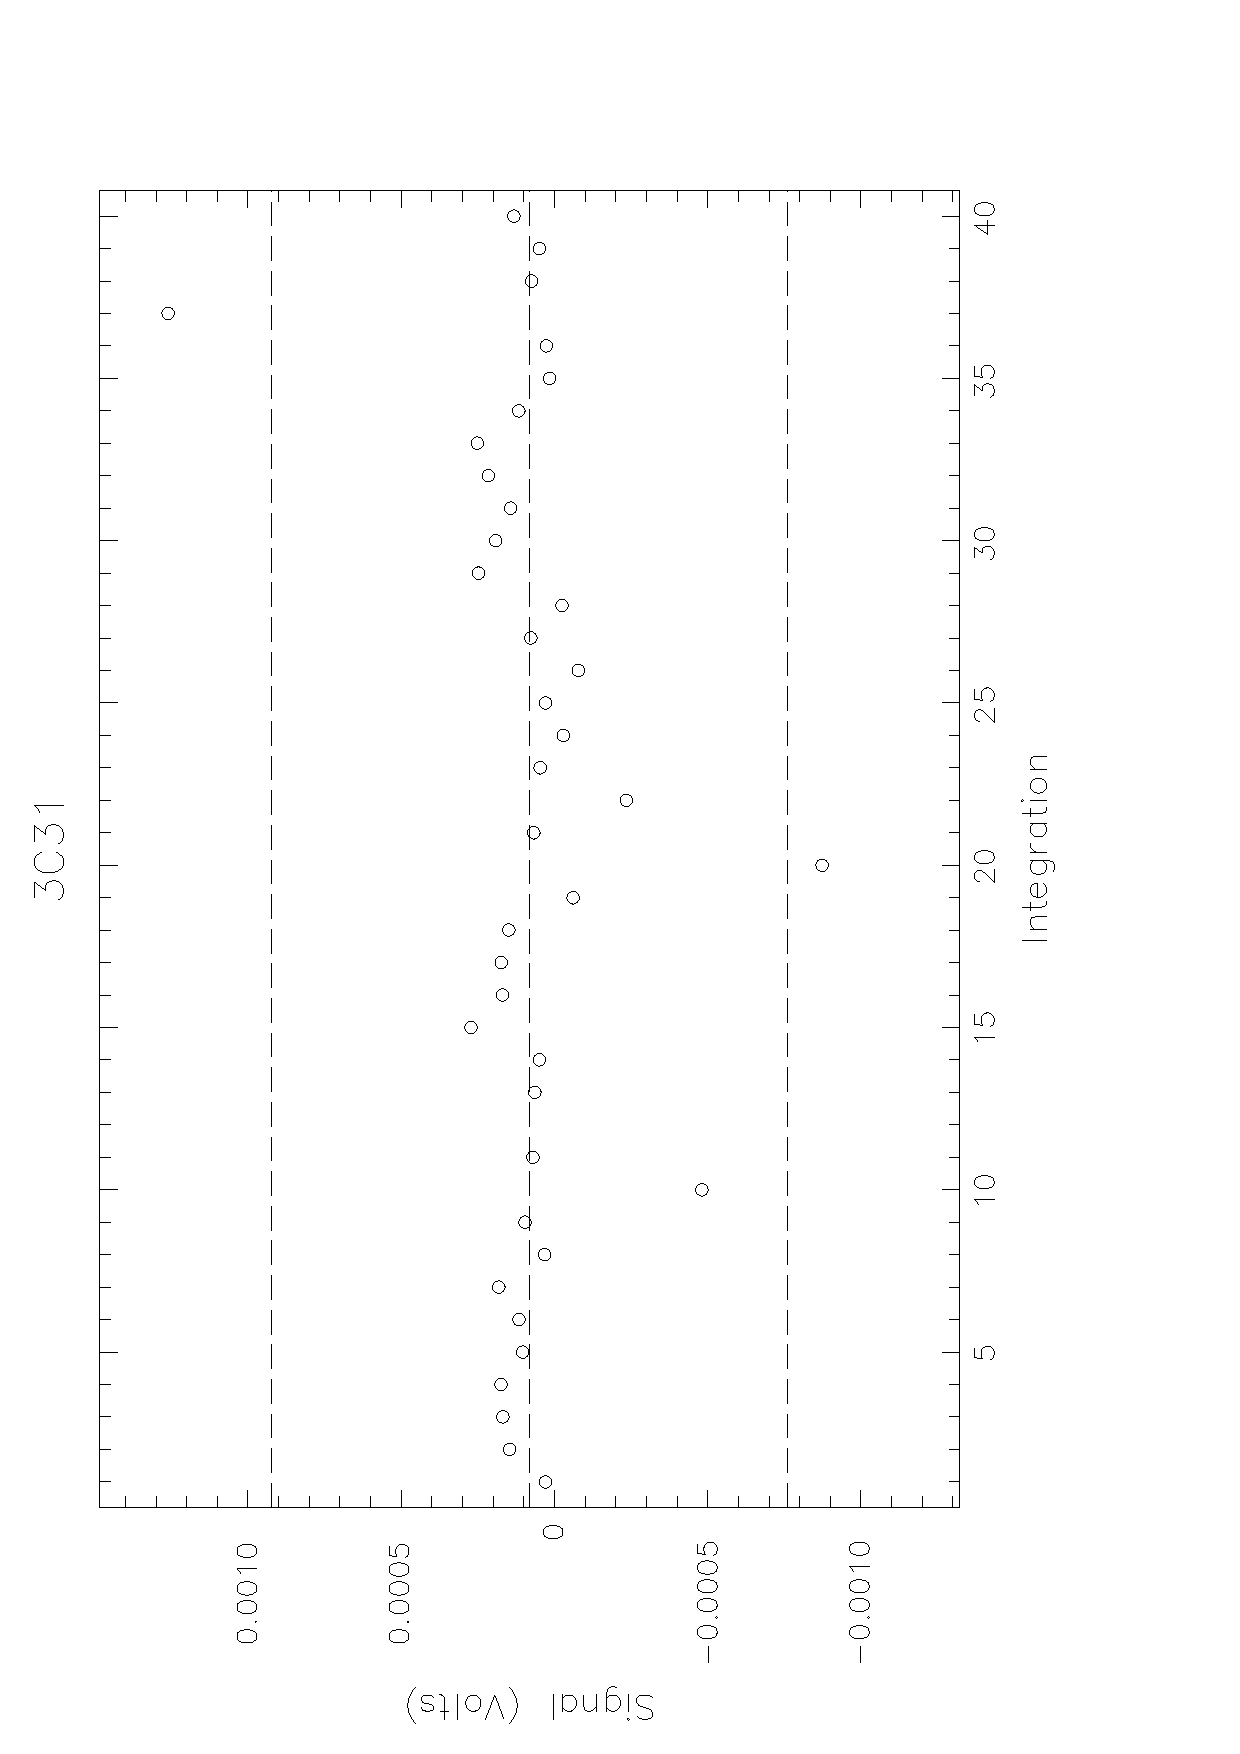
\includegraphics[width=0.9\textwidth]{sc10_fig1}
\end{center}
\caption[Concatenated data for observations \#70 and \#71.]{Concatenated data for
 observations \#70 and \#71. The mean and plus and minus 3$\sigma$
 levels are indicated with the dashed lines.}
\label{f1}
\end{figure}

The same procedure is repeated (not shown here) for \#71 to produce
the file \texttt{red71phot.sdf}. We can then combine the two observations
using \scucat:

\begin{small}
\begin{terminalv}
% scucat
OUT - Rootname of files to contain concatenated data > 3C31_2000
IN - Name of input file containing photometry data > red70_phot
SURF: Found data for the following bolometers: g6
SURF: This is a PHOTOM observation of 3C31. There are 20 integrations
IN - Name of input file containing photometry data /!/ > red71_phot
SURF: Found data for the following bolometers: g6
SURF: This is a PHOTOM observation of 3C31. There are 20 integrations
IN - Name of input file containing photometry data /!/ >
\end{terminalv}
\end{small}

We are now in a position to plot and despike the data (see Figure
\ref{f1}). Note that the bolometer name, g6, will be appended to the file
name giving \texttt{3C31\_2000\_g6.sdf}.

\begin{small}
\begin{terminalv}
% qdraw 3C31_2000_g6 mode=4 device=xwindows
NDF is 3C31_2000_g6
The default values have been adopted for parameter ABSLIM.
Current picture has name: DATA, comment: KAPPA_LINPLOT.
Using /home/jas/scuba/test/3C31_2000_g6 as the input NDF.

      Clip (+/-)         mean          std. deviation    Error in mean
      ----------         ----          --------------    -------------
                      0.800321E-04      0.276960E-03      0.437913E-04
         3.000        0.740715E-04      0.136353E-03      0.221194E-04
\end{terminalv}
\end{small}

Clearly, this data set contains large spikes and the best despiking
strategy is to remove the two biggest spikes that fall outside the
3$\sigma$ levels and then replot the data. For this we use the
\sigclip\ command.

\begin{figure}[t]
\begin{center}
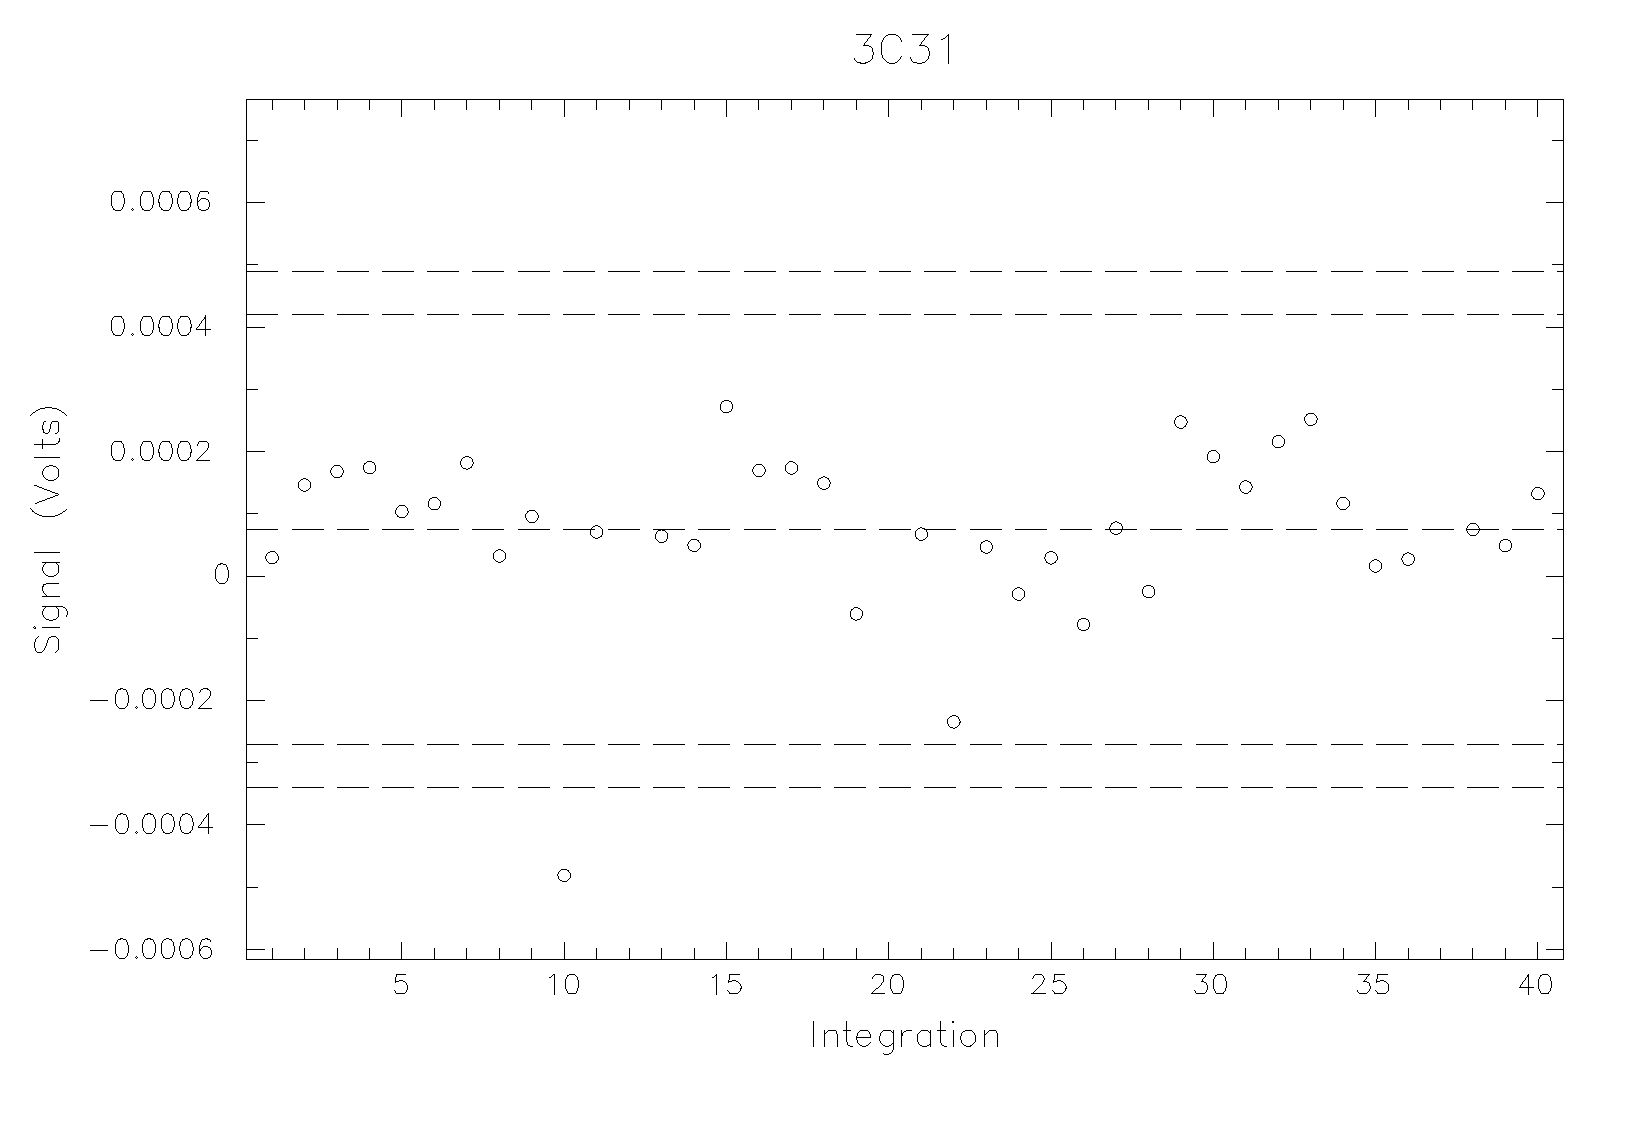
\includegraphics[width=0.9\textwidth]{sc10_fig2}
\end{center}
\caption[Concatenated data after spike removal.]{Concatenated data for \#70 and \#71 after removal of the
two largest spikes with \texttt{sigclip}. The third spike is now excluded
with a 3$\sigma$ clip and there are no further spikes at the 2.5$\sigma$ level.}
\label{f2}
\end{figure}

\begin{small}
\begin{terminalv}
%  sigclip 3C31_2000_g6 3.0
There was 1 element changed in the DATA array below the threshold.
There was 1 element changed in the DATA array above the threshold.
Clipped data written to 3C31_2000_g6_clip.sdf
%  qdraw 3C31_2000_g6_clip device=xwindows mode=4
NDF is 3C31_2000_g6_clip
The default values have been adopted for parameter ABSLIM.
Current picture has name: DATA, comment: KAPPA_LINPLOT.
Using /home/jas/scuba/test/3C31_2000_g6_clip as the input NDF.

      Clip (+/-)         mean          std. deviation    Error in mean
      ----------         ----          --------------    -------------
                      0.740715E-04      0.136353E-03      0.221194E-04
         3.000        0.890766E-04      0.101563E-03      0.166969E-04
%
%  drawsig nsigma=2.5 device=xwindows
Current picture has name: DATA, comment: KAPPA_LINPLOT.
Using /home/jas/scuba/test/3C31_2000_g6_clip as the input NDF.

      Clip (+/-)         mean          std. deviation    Error in mean
      ----------         ----          --------------    -------------
                      0.740715E-04      0.136353E-03      0.221194E-04
         2.500        0.890766E-04      0.101563E-03      0.166969E-04
\end{terminalv}
\end{small}

All three obvious spikes have now been removed and there are no
further spikes down to the 2.5-$\sigma$ level (see Figure~\ref{f2}). The source
is detected at the 5.3-$\sigma$ level.

\subsection{Example reduction - \texttt{scuquick}}

The PERL script \scuquick\ can be used to save time by automating
the reduction process up to and including the \scuphot\ stage.
Note that if many repetitive operations are to be performed then
\scuquick\ (or any other \surf\ command) will take options.
For example,
\begin{terminalv}
% scuquick -remsky
\end{terminalv}
will invoke the \remsky\ command at the appropriate position in
the reduction process. A list of avialable options can be accessed by typing
\begin{small}
\begin{terminalv}
% scuquick -h

Usage:
   scuquick [-h] [-change_flat] [-remsky] [-rebin] [-notau|tau f] [-sub s]
Options:
   -h[elp]       This message
   -quick        Run all tasks with the 'accept' flag (ie take defaults)
   -quiet        Hide all messages generated by the script (note this is
                 not the same as using MSG_FILTER=quiet which hides messages
                 from the tasks)
   -change_flat  Run the change_flatfield task
   -remsky       Run remsky
   -rebin        Regrid the data
   -sub s        Select a specific sub-instrument (else selects all)
   -notau        Use a tau value of 0 in extinction
   -tau f        Use a constant value (f) for the tau. This is dangerous
                 when reducing data containing multiple sub-instruments
                 unless the -sub flag is used.

Notes:
   Parameters for any task can be specified on the command line
   as param=value. All other command line arguments are assumed to be
   input NDFs.
\end{terminalv}
\end{small}

The second example uses \scuquick\ to reduce a long integration on
the radio galaxy 8C1435+635 at 450 and 850$\mu$m. Note that
\scuquick\ will reduce data from both arrays unless instructed
otherwise by use of the \texttt{-sub} option.

This data set was obtained under moderately noisy sky conditions so
sky removal will be used in an attempt to correct for the sky
variations. I'll just reduce the first demodulated data file here.

\begin{small}
\begin{terminalv}
% scuquick -remsky
IN - Name of input file containing demodulated data > 19970502_dem_0052
SURF: run 52 was a PHOTOM observation of object 8C1435+635
USE_CALIBRATOR - Should the data be divided by the internal calibrator /NO/ >
SURF: file contains data for 2 switch(es) in 1 exposure(s) in 40 integration(s)
in 1 measurement(s)
SPIKE_LEVEL - De-spike level /5/ >
OUT - Name of output file to contain reduced switch data > r52
SURF: run 52 was a PHOTOM observation of 8C1435+635
SURF: applying flatfield from photflat1.dat

Processing the LONG sub instrument

SURF: run 52 was a PHOTOM observation with JIGGLE sampling of object 8C1435+635
SURF: file contains data for 1 exposure(s) in 40 integration(s) in 1
measurement(s)
SURF: observation started at sidereal time 14 54 12.45781 and ended at 15 14
46.826715
SURF: file contains data for the following sub-instrument(s)
 - LONG with filter 850
 - SHORT with filter 450
FIRST_TAU - First zenith sky opacity measured > 0.18
FIRST_LST - Sidereal time of first opacity measurement; hh mm ss.ss > 0
SECOND_TAU - Second zenith sky opacity measured > 0.18
SECOND_LST - Sidereal time of second opacity measurement; hh mm ss.ss > 0
Extinction corrected data has been written to file r52_ext_long.sdf
SURF: run 52 was a PHOTOM observation with JIGGLE sampling of object 8C1435+635
BOLOMETERS - The Sky bolometers, [a1,a2] for an array /['d10','c16','c12',
'c2','b9','b10','b11','c5','c16','d10','e2','e3']/ > [h6,h8,h13,h14,g15,g16]
MODE - Sky removal mode /'MEAN'/ >
ITER_SIGMA - Sigma level to drop points from mean iteratively /-1/ > 3.
CLIP - Do you wish to clip the bolometers? /NO/ >
Sky corrected data has been written to file r52_sky_long.sdf
SURF: run 52 was a PHOTOM observation of 8C1435+635
SURF: file contains data for 1 exposure(s) in 40 integrations(s) in 1
measurement(s)
ANALYSIS - Which reduction method /'AVERAGE'/ >
Processed photometry data written to r52_phot_long.sdf and r52_phot_long.dat

Processing the SHORT sub instrument

SURF: run 52 was a PHOTOM observation with JIGGLE sampling of object 8C1435+635
SURF: file contains data for 1 exposure(s) in 40 integration(s) in 1
measurement(s)
SURF: observation started at sidereal time 14 54 12.45781 and ended at 15 14
46.826715
SURF: file contains data for the following sub-instrument(s)
 - LONG with filter 850
 - SHORT with filter 450
FIRST_TAU - First zenith sky opacity measured > 1.0
FIRST_LST - Sidereal time of first opacity measurement; hh mm ss.ss > 0
SECOND_TAU - Second zenith sky opacity measured > 1.0
SECOND_LST - Sidereal time of second opacity measurement; hh mm ss.ss > 0
Extinction corrected data has been written to file r52_ext_short.sdf
SURF: run 52 was a PHOTOM observation with JIGGLE sampling of object 8C1435+635
BOLOMETERS - The Sky bolometers, [a1,a2] for an array /['h6','h8','h13','h14',
'g15','g16']/ > [d10,c16,c12,c2,b9,b10,b11,c5,c16,d10,e2,e3]
MODE - Sky removal mode /'MEAN'/ >
ITER_SIGMA - Sigma level to drop points from mean iteratively /-1/ > 3.
CLIP - Do you wish to clip the bolometers? /NO/ >
Sky corrected data has been written to file r52_sky_short.sdf
SURF: run 52 was a PHOTOM observation of 8C1435+635
SURF: file contains data for 1 exposure(s) in 40 integrations(s) in 1
measurement(s)
ANALYSIS - Which reduction method /'AVERAGE'/ >
Processed photometry data written to r52_phot_short.sdf and r52_phot_short.dat
\end{terminalv}
\end{small}

and similarly for the rest of the data after which \scucat\ and
display/despike procedures can be followed as before. Note that I took
the `default' sky bolometers which correspond to the inner ring of the
long-wave array in this case - in fact these are not strictly the
default but rather the last combination that were used. I recommend
reducing the data both with and without sky removal since under very
stable conditions the signal-to-noise can be degraded by removing the
sky.  A useful aid is a plot of signals from the source bolometer and
sky removal bolometers. There are a variety of ways of doing this:
Appendix A describes how to get ascii output for any bolometer; here
I'll use \surf\ and \Kappa\ commands to investigate the
effects of the adopted sky removal. Firstly, we can use \texttt{scuphot}
and \scucat\ to write out data for all bolometers in a file - in
this case observation \#52 as before. I'll use the extinction
corrected data because these have been processed by \flatf;

\begin{small}
\begin{terminalv}
% scuphot allbols=true
IN - Name of input file containing demodulated data // > r52_ext_long
SURF: run 52 was a PHOTOM observation of 8C1435+635
SURF: file contains data for 1 exposure(s) in 40 integrations(s) in 1
measurement(s)
ANALYSIS - Which reduction method /'AVERAGE'/ >
OUT - Name of container file to hold map and time-sequence data > r52_all
SCUPHOT: All bolometers selected
FILE - Name of ASCII file to contain results summary /!/ > r52_all.dat
% scucat
OUT - Rootname of files to contain concatenated data > r52
IN - Name of input file containing photometry data // > r52_all
SURF: Found data for the following bolometers:
g1,g2,g3,g4,g7,g8,g9,g10,g11,g13,g14,g15,g16,h1,h2,h4,h5,h6,h7,h8,h9,h10,h11,h1
2,h13,h14,h15,h16,i1,i2,i3,i4,i5,i6,i7,i8,i9
SURF: This is a PHOTOM observation of 8C1435+635. There are 40 integrations
IN - Name of input file containing photometry data /!/ >
\end{terminalv}
\end{small}

Each bolometer now has a file called, e.g. \texttt{r52\_h7.sdf}. The
\Kappa\ commands \add\ and \cdiv\ can be used to get a
mean sky value for the inner ring.

\begin{figure}[t]
\begin{center}
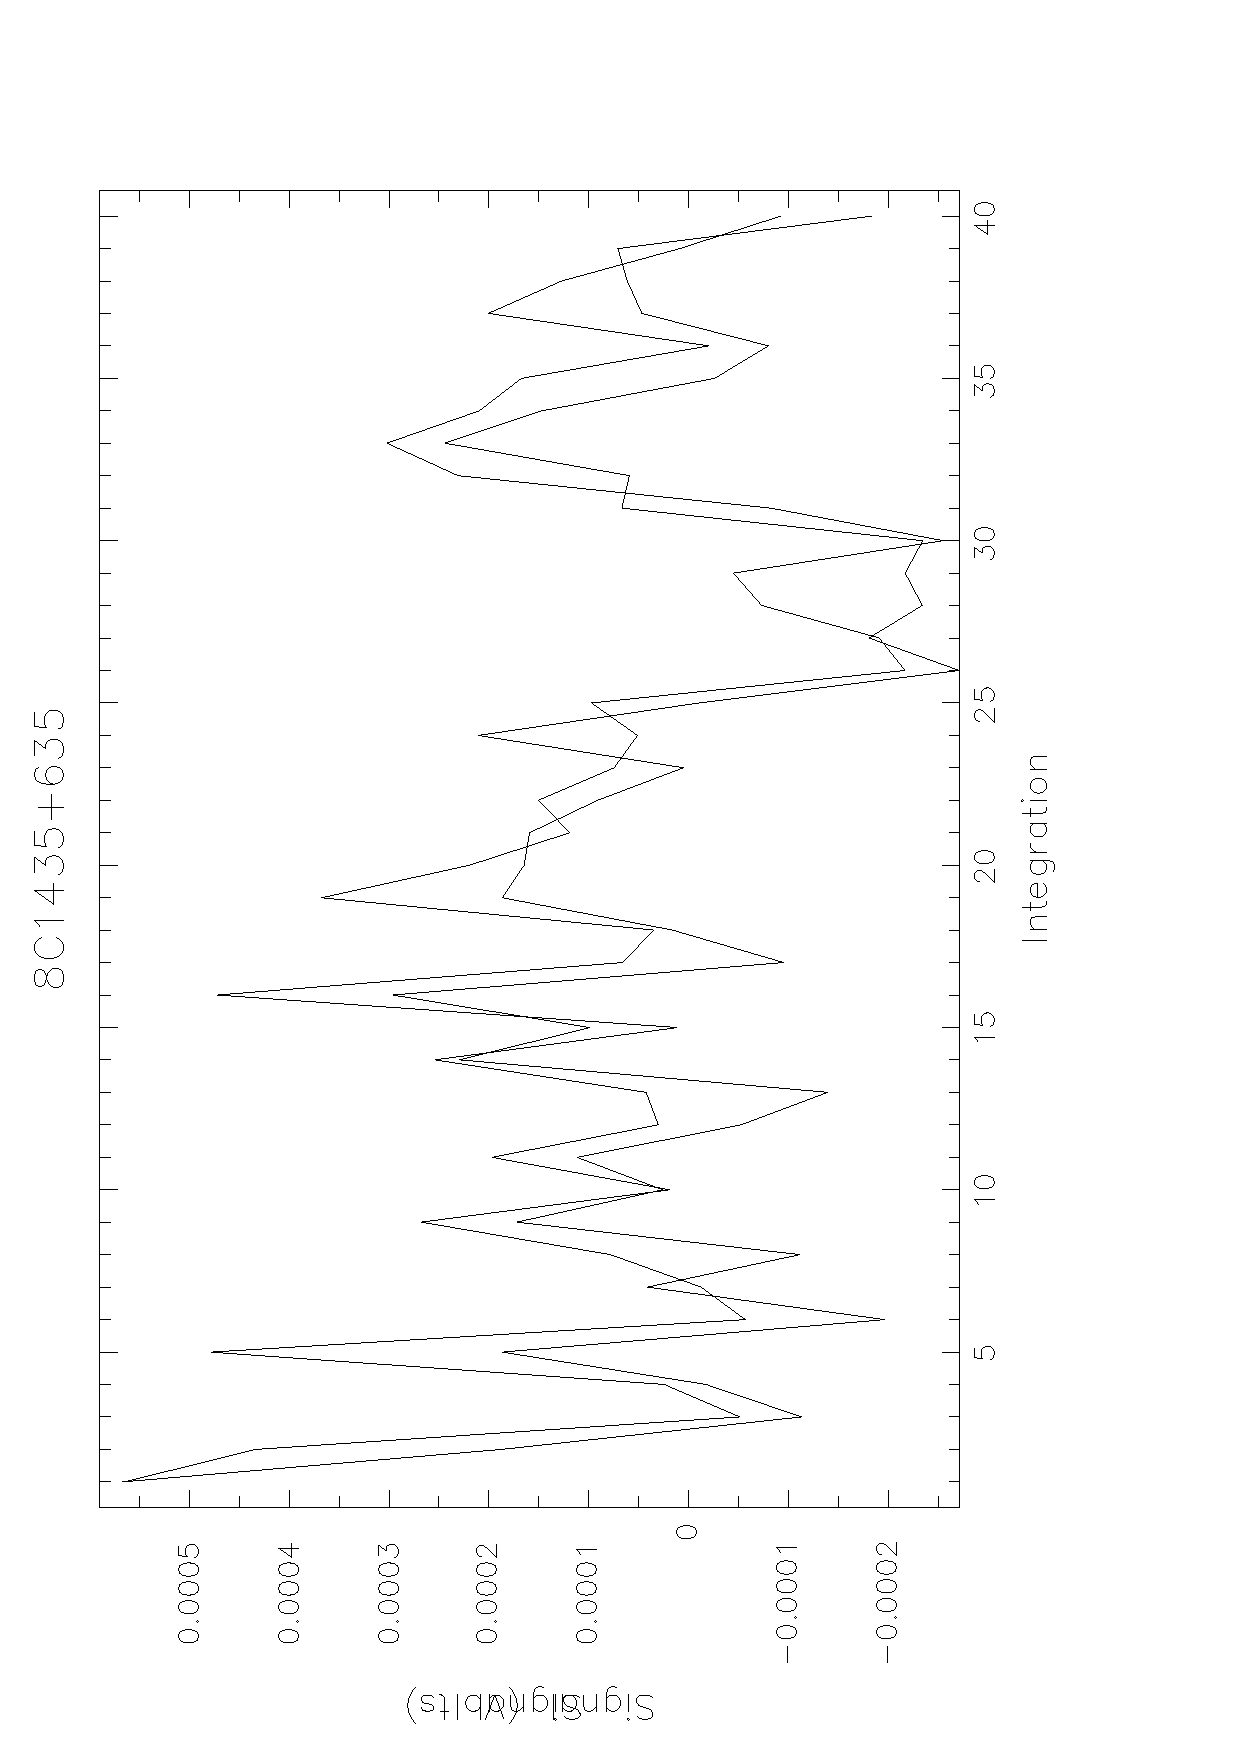
\includegraphics[width=0.9\textwidth]{sc10_fig3}
\end{center}
\caption[Comparison with sky noise.]{Comparison of the the signal from the central bolometer of
the long-wave array with the mean signal from the six surrounding sky
bolometers. Correlated sky noise is clearly seen in this case.}
\label{f3}
\end{figure}

\begin{small}
\begin{terminalv}
% add
IN1 - First input NDF /'r52_all'/ > r52_h6
IN2 - Second input NDF > r52_h8
OUT - Output NDF > sum
% add
IN1 - First input NDF /@sum/ > sum
IN2 - Second input NDF > r52_h13
OUT - Output NDF > sum1
% add
IN1 - First input NDF /@sum1/ > sum1
IN2 - Second input NDF > r52_h14
OUT - Output NDF > sum2
% add
IN1 - First input NDF /@sum2/ >
IN2 - Second input NDF > r52_g15
OUT - Output NDF > sum3
% add
IN1 - First input NDF /sum3/ >
IN2 - Second input NDF > r52_g16
OUT - Output NDF > sum4
% cdiv
IN - Input NDF data structure /@sum4/ >
SCALAR - Division constant /6/ >
OUT - Output NDF > inner_ring
%
\end{terminalv}
\end{small}

and then use \linplot\ to overlay the data (you can use
e.g. lincol=red to get coloured plots),

\begin{terminalv}
% linplot r52_h7 device=xwindows mode=line
% linplot inner_ring device=xwindows mode=line noclear
\end{terminalv}

Figure \ref{f3} shows the output from \linplot\ which clearly shows that
the signal and sky are correlated in this case.

\section{\xlabel{twobol}Two and three bolometer chopping\label{twobol}}

It is possible to chop between two or three bolometers on the array,
the main benefit being more time spent on-source during the
observation. The reduction of these data is very similar to the single
bolometer method shown in the preceeding section. The only
recognizable difference is that \scucat\ will produce a
concatenated output file for each bolometer. For example, if data were
taken simultaneously with the long-wavelength array pixels h7 and h9
and the specified output file is \texttt{source1} then files \texttt{source1\_h7.sdf} and \texttt{source1\_h9.sdf} will result.

The most robust method of reducing these data is to observe a planet,
such as Mars, in exactly the same way and then to calibrate each
bolometer separately into flux units. The coadded result and its
statistical uncertainty can then be calculated with standard formulae.

\section{Is it correct to coadd the data sets? The K-S test}

Photometric observations of faint sources often require that the
source be observed for long periods, during which the atmospheric
conditions and/or telescope related parameters such as pointing and
focus may vary. These effects are particularly noticeable around
sunrise and sunset, for example. The consistency of the entire data
set can be investigated with the use of a two sample
Kolmogorov-Smirnov (KS) test. Again, the method adopted for the SCUBA
data reduction package is analogous to that used previously by COADD
for UKT14 \cite{dhh}.

The data set is split into subsamples that are specified by the
user. The size of these subsamples clearly depends on the total number
of photometric points and some experimentation is required but, for
example, if the data set consists of 100 points then subsamples of 20
would be a sensible choice. The first subsample is compared with the
second and is `rejected' if the probability that the two are
statistically different is lower than a user specified tolerance. If
the KS test returns 0.1 then this indicates that there is a 90\%
probability that the two samples are different. If the first two
subsamples are consistent then they are concatenated and compared with
the third etc, otherwise the first subsample is compared with the
third and so on. A problem arises if, for some reason, the first
subsample is different from each of the others since in this case most
of the data set will be rejected. If this happens it is necessary to
repeat the process but this time select a different subsample against
which the others are to be compared. In general, it is good practice
to change the order and repeat the test.

The best way to illustrate the whole process is with an example using
real data.

\subsection{An example}

For the example I'll use the 8C1435+635 measurement at 850$\mu$m that was
discussed in \S 4.2. Here the whole data set has been reduced with sky
removal, concatenated and despiked using \sigclip\ (see Figure~\ref{f4}). Note
that \sigclip\ must be used rather than \drawsig\ because it produces an
output file devoid of spikes. I renamed this file 8c\_clip for brevity.

\begin{figure}[t]
\begin{center}
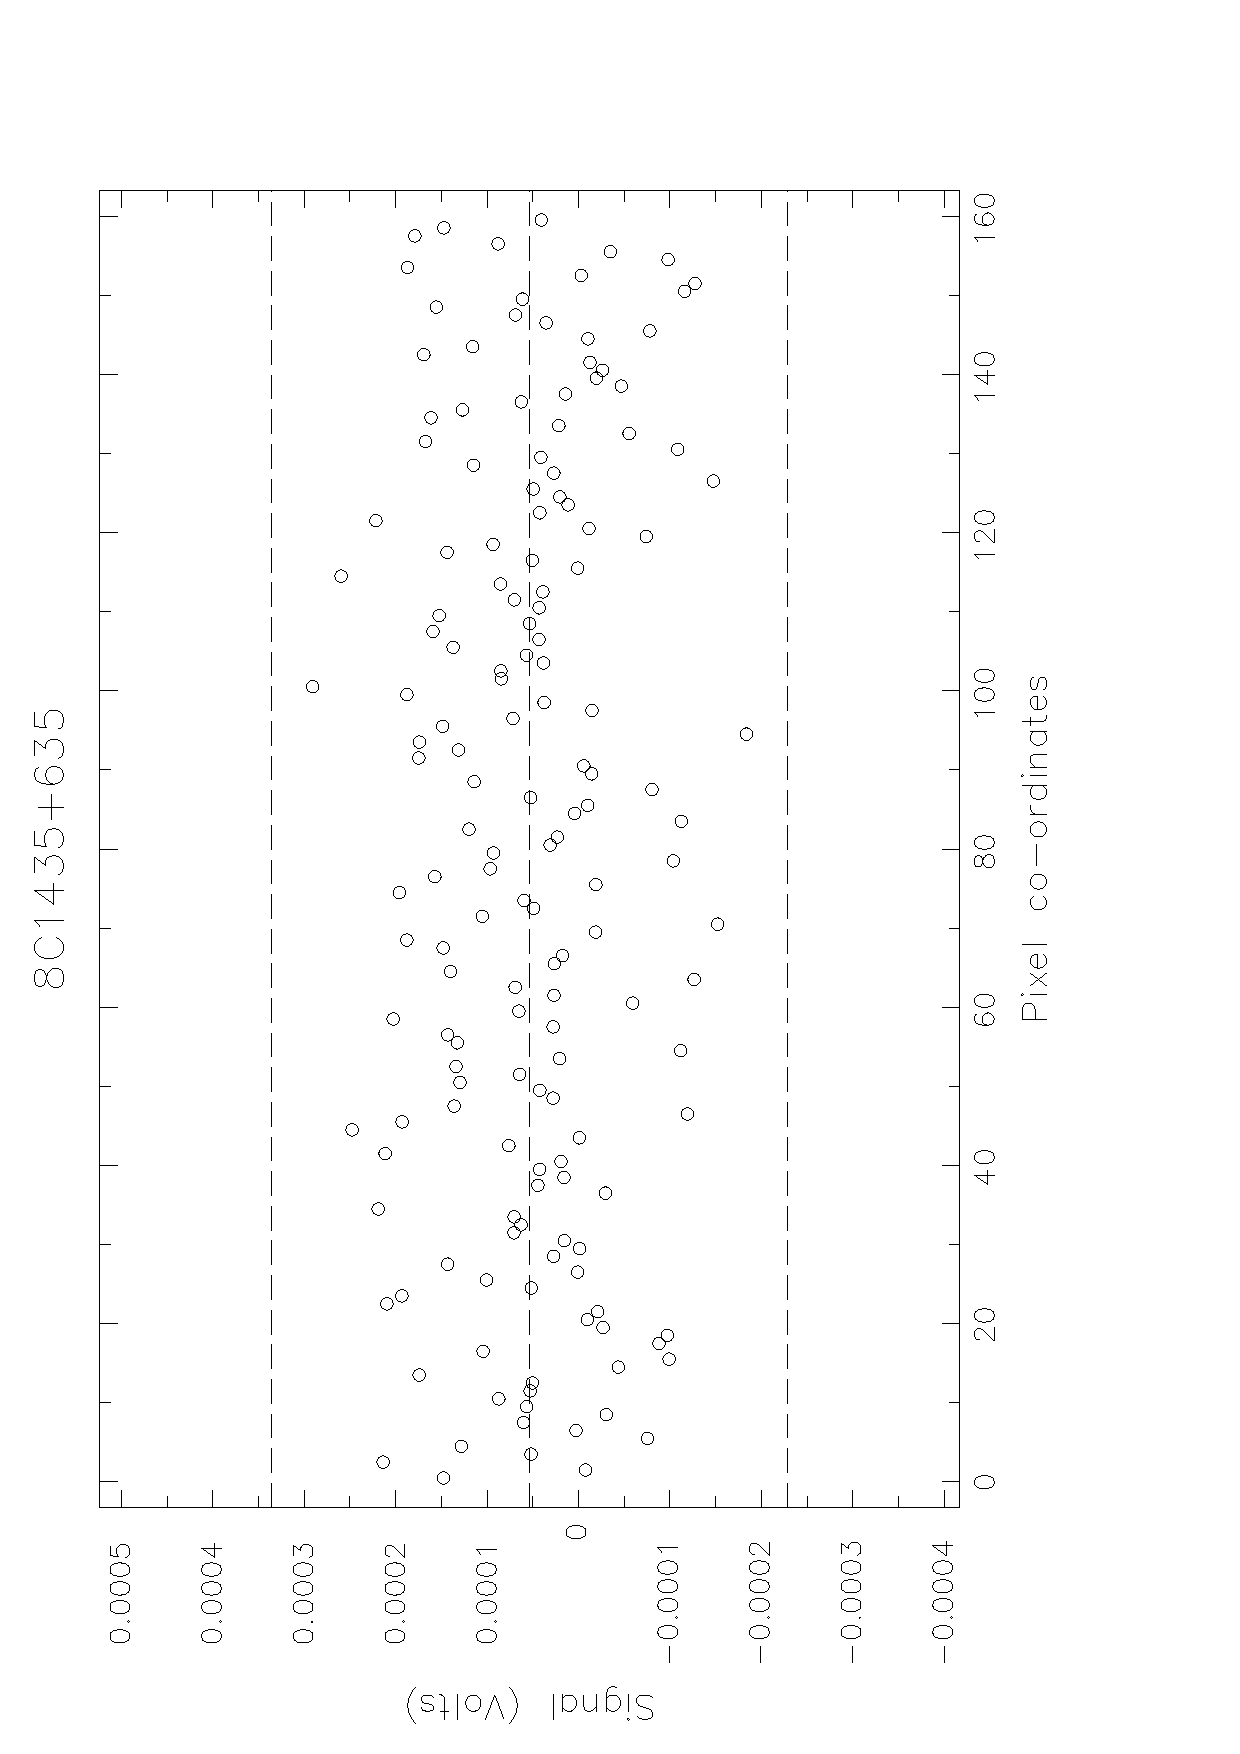
\includegraphics[width=0.9\textwidth]{sc10_fig4}
\end{center}
\caption[A 48 minute integration on 8C1435+635]{A 48 minute (160 x 9/2.0 jiggle patterns) integration on
8C1435+635. The \sigclip\ command has been used to produce a
dataset despiked at the 3$\sigma$ level.}
\label{f4}
\end{figure}

The \kstest\ command is part of the \starlink\
\Kappa\ package and
takes a variety of parameters. In this document I'll just discuss those
relevant to the basic KS test as applicable to photometry data. A full
description of the routine can be found in the \Kappa\ manual
(\xref{SUN/95}{sun95}{}).

I'll split the dataset into subsamples of 20 integrations (the second
subsample will contain only 19 points because sigclip removed one
spike). In this example, the input and output file names are specified
on the command line but this need not be the case.  Note that it is,
however, necessary to give the number of samples and the probability
in the same way, otherwise the default values of 3 and 0.05 are
assumed respectively. A maximum number of 20 subsamples is allowed by
\kstest.

\begin{small}
\begin{terminalv}
% kstest in=8c_clip out=8c_ks nsample=8 limit=0.05
Data for "8C1435+635" contain 20 points, of which 20 are good.
Data for "8C1435+635" contain 20 points, of which 19 are good.
Data for "8C1435+635" contain 20 points, of which 20 are good.
Data for "8C1435+635" contain 20 points, of which 20 are good.
Data for "8C1435+635" contain 20 points, of which 20 are good.
Data for "8C1435+635" contain 20 points, of which 20 are good.
Data for "8C1435+635" contain 20 points, of which 20 are good.
Data for "8C1435+635" contain 20 points, of which 20 are good.

                  Probability        Max. Sep.
--------------------------------------------------------------
 cf. with   2 :   0.288655E+00       0.300000E+00  (Accepted)
 cf. with   3 :   0.244933E+00       0.270513E+00  (Accepted)
 cf. with   4 :   0.981682E+00       0.116102E+00  (Accepted)
 cf. with   5 :   0.924850E+00       0.132279E+00  (Accepted)
 cf. with   6 :   0.288812E-01       0.344444E+00  (Rejected)
 cf. with   7 :   0.380108E+00       0.215151E+00  (Accepted)
 cf. with   8 :   0.583820E+00       0.181092E+00  (Accepted)

Number of subsamples rejected: 1
Coadded result is 4.8022197E-5 +/- 8.0190266E-6
\end{terminalv}
\end{small}

Subsample 6 which contains many more points with a signal greater than
zero compared to the other subsamples is rejected (see Figure~\ref{f4}).  If
you wish to view the truncated dataset then 8c\_ks.sdf can be
displayed with \qdraw\ in the usual way.

If the first sample is anomalous then we can repeat the test in
reverse order by applying the \Kappa\ command \flip\ to the
original dataset, 8c\_clip;

\begin{terminalv}
% flip 8c_clip 8c_flip
\end{terminalv}
More generally, any subsample can be specified with a
\xref{NDF section}{sun33}{ndf_sections} \cite{ndf}. In the above
example, subsample 7 is 8c\_clip(121:140). The \kstest\ command can then
read in an ascii file containing a list of NDF sections, such as,

\begin{small}
\begin{terminalv}
% cat kstest.dat
8c_clip(121:140)
8c_clip(1:20)
8c_clip(61:80)
8c_clip(81:100)
8c_clip(21:40)
8c_clip(101:120)
8c_clip(141:160)
8c_clip(41:60)
%
\end{terminalv}
\end{small}

The following command then performs the KS test using this file;

\begin{small}
\begin{terminalv}
% kstest '^kstest.dat' out=8c_ks limit=0.05
Data for "8C1435+635" contain 20 points, of which 20 are good.
Data for "8C1435+635" contain 20 points, of which 20 are good.
Data for "8C1435+635" contain 20 points, of which 20 are good.
Data for "8C1435+635" contain 20 points, of which 20 are good.
Data for "8C1435+635" contain 20 points, of which 19 are good.
Data for "8C1435+635" contain 20 points, of which 20 are good.
Data for "8C1435+635" contain 20 points, of which 20 are good.
Data for "8C1435+635" contain 20 points, of which 20 are good.

                  Probability        Max. Sep.
--------------------------------------------------------------
 cf. with   2 :   0.497342E+00       0.250000E+00  (Accepted)
 cf. with   3 :   0.767976E+00       0.175000E+00  (Accepted)
 cf. with   4 :   0.860007E+00       0.150000E+00  (Accepted)
 cf. with   5 :   0.444130E+00       0.212500E+00  (Accepted)
 cf. with   6 :   0.100815E-01       0.384849E+00  (Rejected)
 cf. with   7 :   0.835178E+00       0.146970E+00  (Accepted)
 cf. with   8 :   0.189298E+00       0.253361E+00  (Accepted)

Number of subsamples rejected: 1
Coadded result is 4.8022197E-5 +/- 8.0190266E-6

%
\end{terminalv}
\end{small}
Note that the \param{NSAMPLE} parameter is now redundant and also that single
quotes must surround the input file name. The final result in this case
is unchanged, of course.

\section{A note on calibration}

To get the final calibrated flux in Jy we need to multiply by a conversion
factor or responsivity that is calculated by making observations of a compact
planet such as Mars or Uranus; the planetary fluxes, corrected for the SCUBA
beamsizes, are available from the \starlink\ package \fluxes\
(\xref{SUN/213}{sun213}{}) \cite{fluxes}. Note that the secondary sources used
for the calibration of UKT14 photometry \cite{uktphot} will probably have
different fluxes in the SCUBA wavebands, mainly due to the different beam
sizes, i.e.\ these sources are extended at some level. This is certainly the
case for the one source, N2071IR, that has been calibrated against a planet so
far and the whole list may have to be re-observed.




\appendix
\section{Getting ASCII output}

ASCII output can be produced for any bolometer using the \ndfascii\ command
which is part of the \starlink\ package, \convert.  Note that if you intend
to compare the bolometer signals then the flatfielded or extinction corrected
data must be used. Here's observation \#52 of 8C1435+635 again,

\begin{small}
\begin{terminalv}
% convert

   CONVERT commands are now available -- (Version 0.6-2, 1996 September)

   Defaults for automatic NDF conversion are set.

   Type conhelp for help on CONVERT commands.

% ndf2ascii prompt
IN - Input NDF data structure /@red52_phot/ > red52_ext(19,,2)
COMP - Array component to copy to the ASCII file /'Data'/ >
FITS - Write a FITS header in the ASCII file? /NO/ >
FIXED - Fixed format of the array values? /NO/ > y
NOPEREC - Number of data values per ASCII record /1/ >
OUT - ASCII file /@h14_52/ > h7_52
%
\end{terminalv}
\end{small}

The output file \texttt{h7\_52} contains a single column of numbers each
corresponding to 2 seconds of integration time (corrected for the
beam-switching). The input NDF, red52\_ext(19,,2) is thus the output
of \ext\ but using a section to select the central pixel of
the long-wave array, i.e. bolometer 19.  The `2' just selects the
central beam position. Similarly the sky bolometer, h14, is referred
to as red52(26,,2). Further information on the data structure can be
found in the \surf\ documentation (\xref{SUN/216}{sun216}{}).

%%%%%%%%%%%%%%%%%%%%%%%%%%%%%%%%%%%%%%%%%%%%%%%%%%%%%%%%
%%%%%%% End of document
% Do you want an index?
%\printindex


\clearpage
\begin{thebibliography}{}
\addcontentsline{toc}{section}{References}

\bibitem{obsguide}
Gear~W.~K., Holland~W.~S., Lightfoot~J.~F., 1997
\textit{SCUBA Observing Manual}, \htmladdnormallink{SCUBA System Note
1}{http://www.jach.hawaii.edu/jcmt_sw/scuba/}, (see also the SCUBA software homepage:
\htmladdnormallink{http://www.jach.hawaii.edu/jcmt\_sw/scuba/}{http://www.jach.hawaii.edu/jcmt_sw/scuba/})


\bibitem{ukt14}
Duncan~W.~D., Robson~E.~I., Ade~P.~A.~R., Griffin~M.~J., Sandell~G., 1990,
\textit{MNRAS}, \textbf{243}, 126

\bibitem{surf}
Jenness~T., Lightfoot~J.~F., 1997, \textit{SURF -- SCUBA User Reduction Facility},
\xref{Starlink User Note 216}{sun216}{} (see also the SURF homepage:
\htmladdnormallink{http://www.jach.hawaii.edu/jcmt\_sw/scuba/surf/}{http://www.jach.hawaii.edu/jcmt_sw/scuba/surf/})

\bibitem{kappa}
Currie~M.~J., 1997, \textit{KAPPA --- Kernel Application Package},
\xref{Starlink User Note 95}{sun95}{}

\bibitem{convert}
Currie~M.~J., Privett~G.~J., Chipperfield~A.~J., 1995 \textit{CONVERT --
A format-conversion package}, \xref{Starlink User Note 55}{sun55}{}

\bibitem{perl}
Wall~L., Christiansen~T., Schwartz~R.~L., 1996,
\htmladdnormallink{\textit{Programming Perl}}{http://www.perl.org/}, 2nd
edn., \htmladdnormallink{O'Reilly \& Associates, Inc.}{http://www.ora.com/}

\bibitem{dhh}
Hughes~D.~H., 1993, \textit{JCMT--UKIRT Newsletter}, \textbf{4}, 32

\bibitem{ndf}
Warren-Smith~R.~F., 1995, \textit{NDF -- Routines for Accessing the Extensible
N-Dimensional Data Format}, \xref{Starlink User Note 33}{sun33}{}

\bibitem{fluxes}
Privett~G.~J., Jenness~T., Matthews~H.~E., 1997, \textit{FLUXES --
JCMT Position and Flux Density Calibration},
\xref{Starlink User Note 213}{sun213}{}

\bibitem{uktphot}
Sandell~G., 1994, \textit{MNRAS}, \textbf{271}, 75

\end{thebibliography}


\end{document}
